\documentclass[tikz,border=7pt]{standalone}
\usepackage[T1]{fontenc}
\usepackage[scaled=0.95]{helvet}
\renewcommand{\familydefault}{\sfdefault}
\usetikzlibrary{arrows.meta,calc}

\definecolor{ink}{HTML}{202733}
\definecolor{muted}{HTML}{697386}
\definecolor{rule}{HTML}{D3D9E2}
\definecolor{panel}{HTML}{F7F8FA}
\definecolor{structure}{HTML}{405FB5}
\definecolor{metadata}{HTML}{B85D3D}

\begin{document}
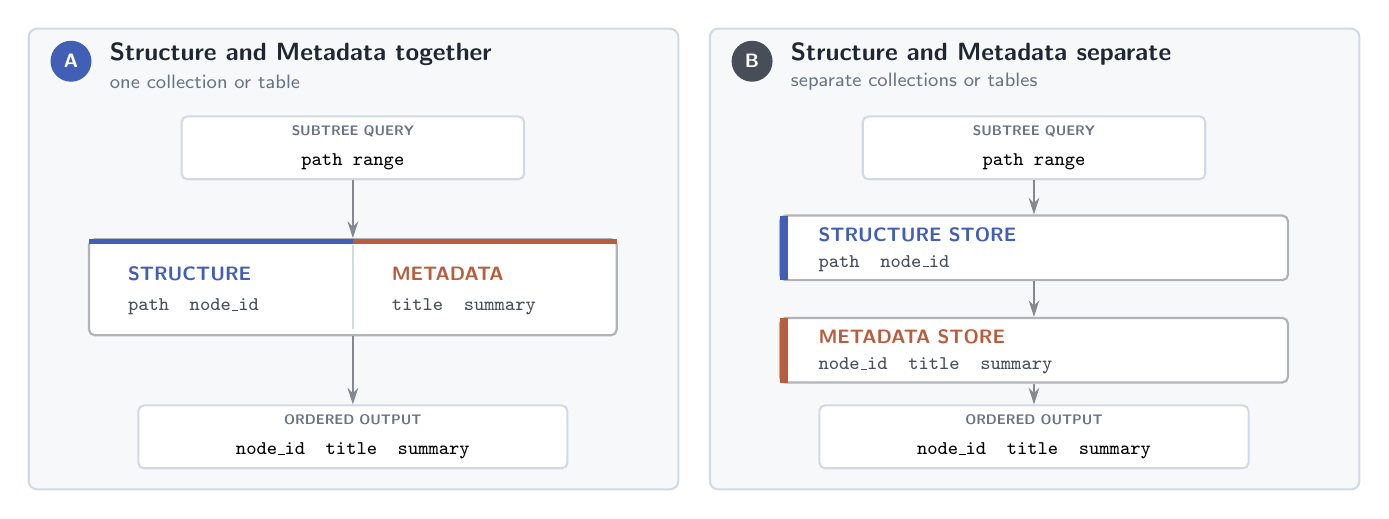
\begin{tikzpicture}[
  x=1cm,y=1cm,
  flow/.style={-{Stealth[length=2.1mm,width=1.35mm]}, draw=ink!55,
    line width=0.85pt},
  panelbox/.style={draw=rule, fill=panel, rounded corners=3pt,
    line width=0.75pt},
  endpoint/.style={draw=rule, fill=white, rounded corners=2pt,
    line width=0.75pt, align=center},
  store/.style={draw=ink!35, fill=white, rounded corners=2pt,
    line width=0.8pt}
]

% Balanced panels with generous vertical rhythm.
\node[panelbox, minimum width=8.25cm, minimum height=5.85cm,
  anchor=south west] at (0,0.20) {};
\node[panelbox, minimum width=8.25cm, minimum height=5.85cm,
  anchor=south west] at (8.65,0.20) {};

% Panel titles.
\node[circle, fill=structure, text=white, minimum size=5.2mm,
  inner sep=0pt, font=\scriptsize\bfseries] at (0.55,5.65) {A};
\node[anchor=west, font=\small\bfseries, text=ink] at (0.92,5.74)
  {Structure and Metadata together};
\node[anchor=west, font=\scriptsize, text=muted] at (0.92,5.39)
  {one collection or table};

\node[circle, fill=ink!82, text=white, minimum size=5.2mm,
  inner sep=0pt, font=\scriptsize\bfseries] at (9.20,5.65) {B};
\node[anchor=west, font=\small\bfseries, text=ink] at (9.57,5.74)
  {Structure and Metadata separate};
\node[anchor=west, font=\scriptsize, text=muted] at (9.57,5.39)
  {separate collections or tables};

% Shared endpoints.  Labels are inside boxes, never on connector lines.
\node[endpoint, minimum width=4.35cm, minimum height=7.2mm]
  (queryA) at (4.13,4.55) {
    {\tiny\bfseries\color{muted} SUBTREE QUERY}\\[-1pt]
    {\scriptsize\ttfamily path range}};
\node[endpoint, minimum width=4.35cm, minimum height=7.2mm]
  (queryB) at (12.78,4.55) {
    {\tiny\bfseries\color{muted} SUBTREE QUERY}\\[-1pt]
    {\scriptsize\ttfamily path range}};

\node[endpoint, minimum width=5.45cm, minimum height=7.2mm]
  (rowsA) at (4.13,0.88) {
    {\tiny\bfseries\color{muted} ORDERED OUTPUT}\\[-1pt]
    {\scriptsize\ttfamily node\_id\quad title\quad summary}};
\node[endpoint, minimum width=5.45cm, minimum height=7.2mm]
  (rowsB) at (12.78,0.88) {
    {\tiny\bfseries\color{muted} ORDERED OUTPUT}\\[-1pt]
    {\scriptsize\ttfamily node\_id\quad title\quad summary}};

% Layout A: both field groups live inside one physical boundary.
\node[store, minimum width=6.70cm, minimum height=1.22cm]
  (combined) at (4.13,2.78) {};
\fill[structure]
  ([xshift=-3.35cm,yshift=0.61cm]combined.center)
  rectangle ([xshift=0cm,yshift=0.55cm]combined.center);
\fill[metadata]
  ([xshift=0cm,yshift=0.61cm]combined.center)
  rectangle ([xshift=3.35cm,yshift=0.55cm]combined.center);
\draw[rule, line width=0.7pt]
  ([yshift=-0.53cm]combined.center) -- ([yshift=0.53cm]combined.center);

\node[anchor=west, font=\scriptsize\bfseries, text=structure]
  at ([xshift=-2.98cm,yshift=0.17cm]combined.center) {STRUCTURE};
\node[anchor=west, font=\scriptsize\ttfamily, text=ink!82]
  at ([xshift=-2.98cm,yshift=-0.25cm]combined.center)
  {path\quad node\_id};
\node[anchor=west, font=\scriptsize\bfseries, text=metadata]
  at ([xshift=0.37cm,yshift=0.17cm]combined.center) {METADATA};
\node[anchor=west, font=\scriptsize\ttfamily, text=ink!82]
  at ([xshift=0.37cm,yshift=-0.25cm]combined.center)
  {title\quad summary};

\draw[flow] (queryA.south) -- (combined.north);
\draw[flow] (combined.south) -- (rowsA.north);

% Layout B: separate physical boundaries, arranged as a clear three-stage flow.
\node[store, minimum width=6.45cm, minimum height=8.2mm]
  (structureB) at (12.78,3.28) {};
\fill[structure]
  ([xshift=-3.225cm,yshift=0.41cm]structureB.center)
  rectangle ([xshift=-3.13cm,yshift=-0.41cm]structureB.center);
\node[anchor=west, font=\scriptsize\bfseries, text=structure]
  at ([xshift=-2.86cm,yshift=0.17cm]structureB.center)
  {STRUCTURE STORE};
\node[anchor=west, font=\scriptsize\ttfamily, text=ink!82]
  at ([xshift=-2.86cm,yshift=-0.20cm]structureB.center)
  {path\quad node\_id};

\node[store, minimum width=6.45cm, minimum height=8.2mm]
  (metadataB) at (12.78,1.98) {};
\fill[metadata]
  ([xshift=-3.225cm,yshift=0.41cm]metadataB.center)
  rectangle ([xshift=-3.13cm,yshift=-0.41cm]metadataB.center);
\node[anchor=west, font=\scriptsize\bfseries, text=metadata]
  at ([xshift=-2.86cm,yshift=0.17cm]metadataB.center)
  {METADATA STORE};
\node[anchor=west, font=\scriptsize\ttfamily, text=ink!82]
  at ([xshift=-2.86cm,yshift=-0.20cm]metadataB.center)
  {node\_id\quad title\quad summary};

\draw[flow] (queryB.south) -- (structureB.north);
\draw[flow] (structureB.south) -- (metadataB.north);
\draw[flow] (metadataB.south) -- (rowsB.north);

\end{tikzpicture}
\end{document}
